\subsection*{Log ind}
Log ind-funktionen inddeles i en klasse af typen boundary samt en tilhørende controller. Disse fremgår af \autoref{fig:Designlogind}. 

\begin{figure} [H]
\centering
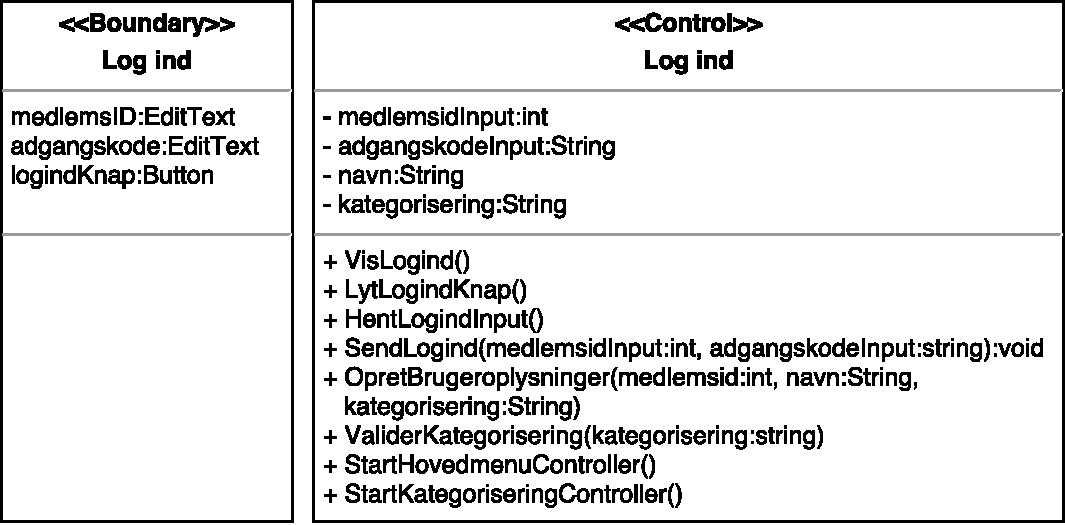
\includegraphics[width=0.5\textwidth]{figures/MVC/MVCLogInd}
\caption{Designklasser for log ind. Til venstre ses grænsefladen og til højre den tilhørende controller.}
\label{fig:Designlogind}
\end{figure}

\noindent
I grænsefladen for \textit{Logind} opstilles tekstfelter af typen EditText, hvor brugeren kan angive medlemsID samt adgangskode. Dertil opsættes en LogindKnap, af typen Button, der ved tryk indikerer, at brugerens informationer er angivet og klar til at logge ind. 

Til denne grænseflade er der opstillet en \textit{Logind} controller. Denne controller har metoderne Vis, Lyt, Hent, Opret, Send, Valider, Start og makeText. Metoden makeText anvendes til at fejlmeddelelser. Controlleren validerer log ind og opretter en entity, hvori oplysninger senere kan lagres. Denne entity beskrives af \autoref{sec:entity}. Ligeledes håndterer controlleren, hvilken grænseflade systemet efterfølgende skal henvises til. Der er i sammenspil med disse designklasser udarbejdet et sekvensdiagram, der fremgår af \autoref{fig:SEKlogind}.

\begin{figure} [H]
\centering
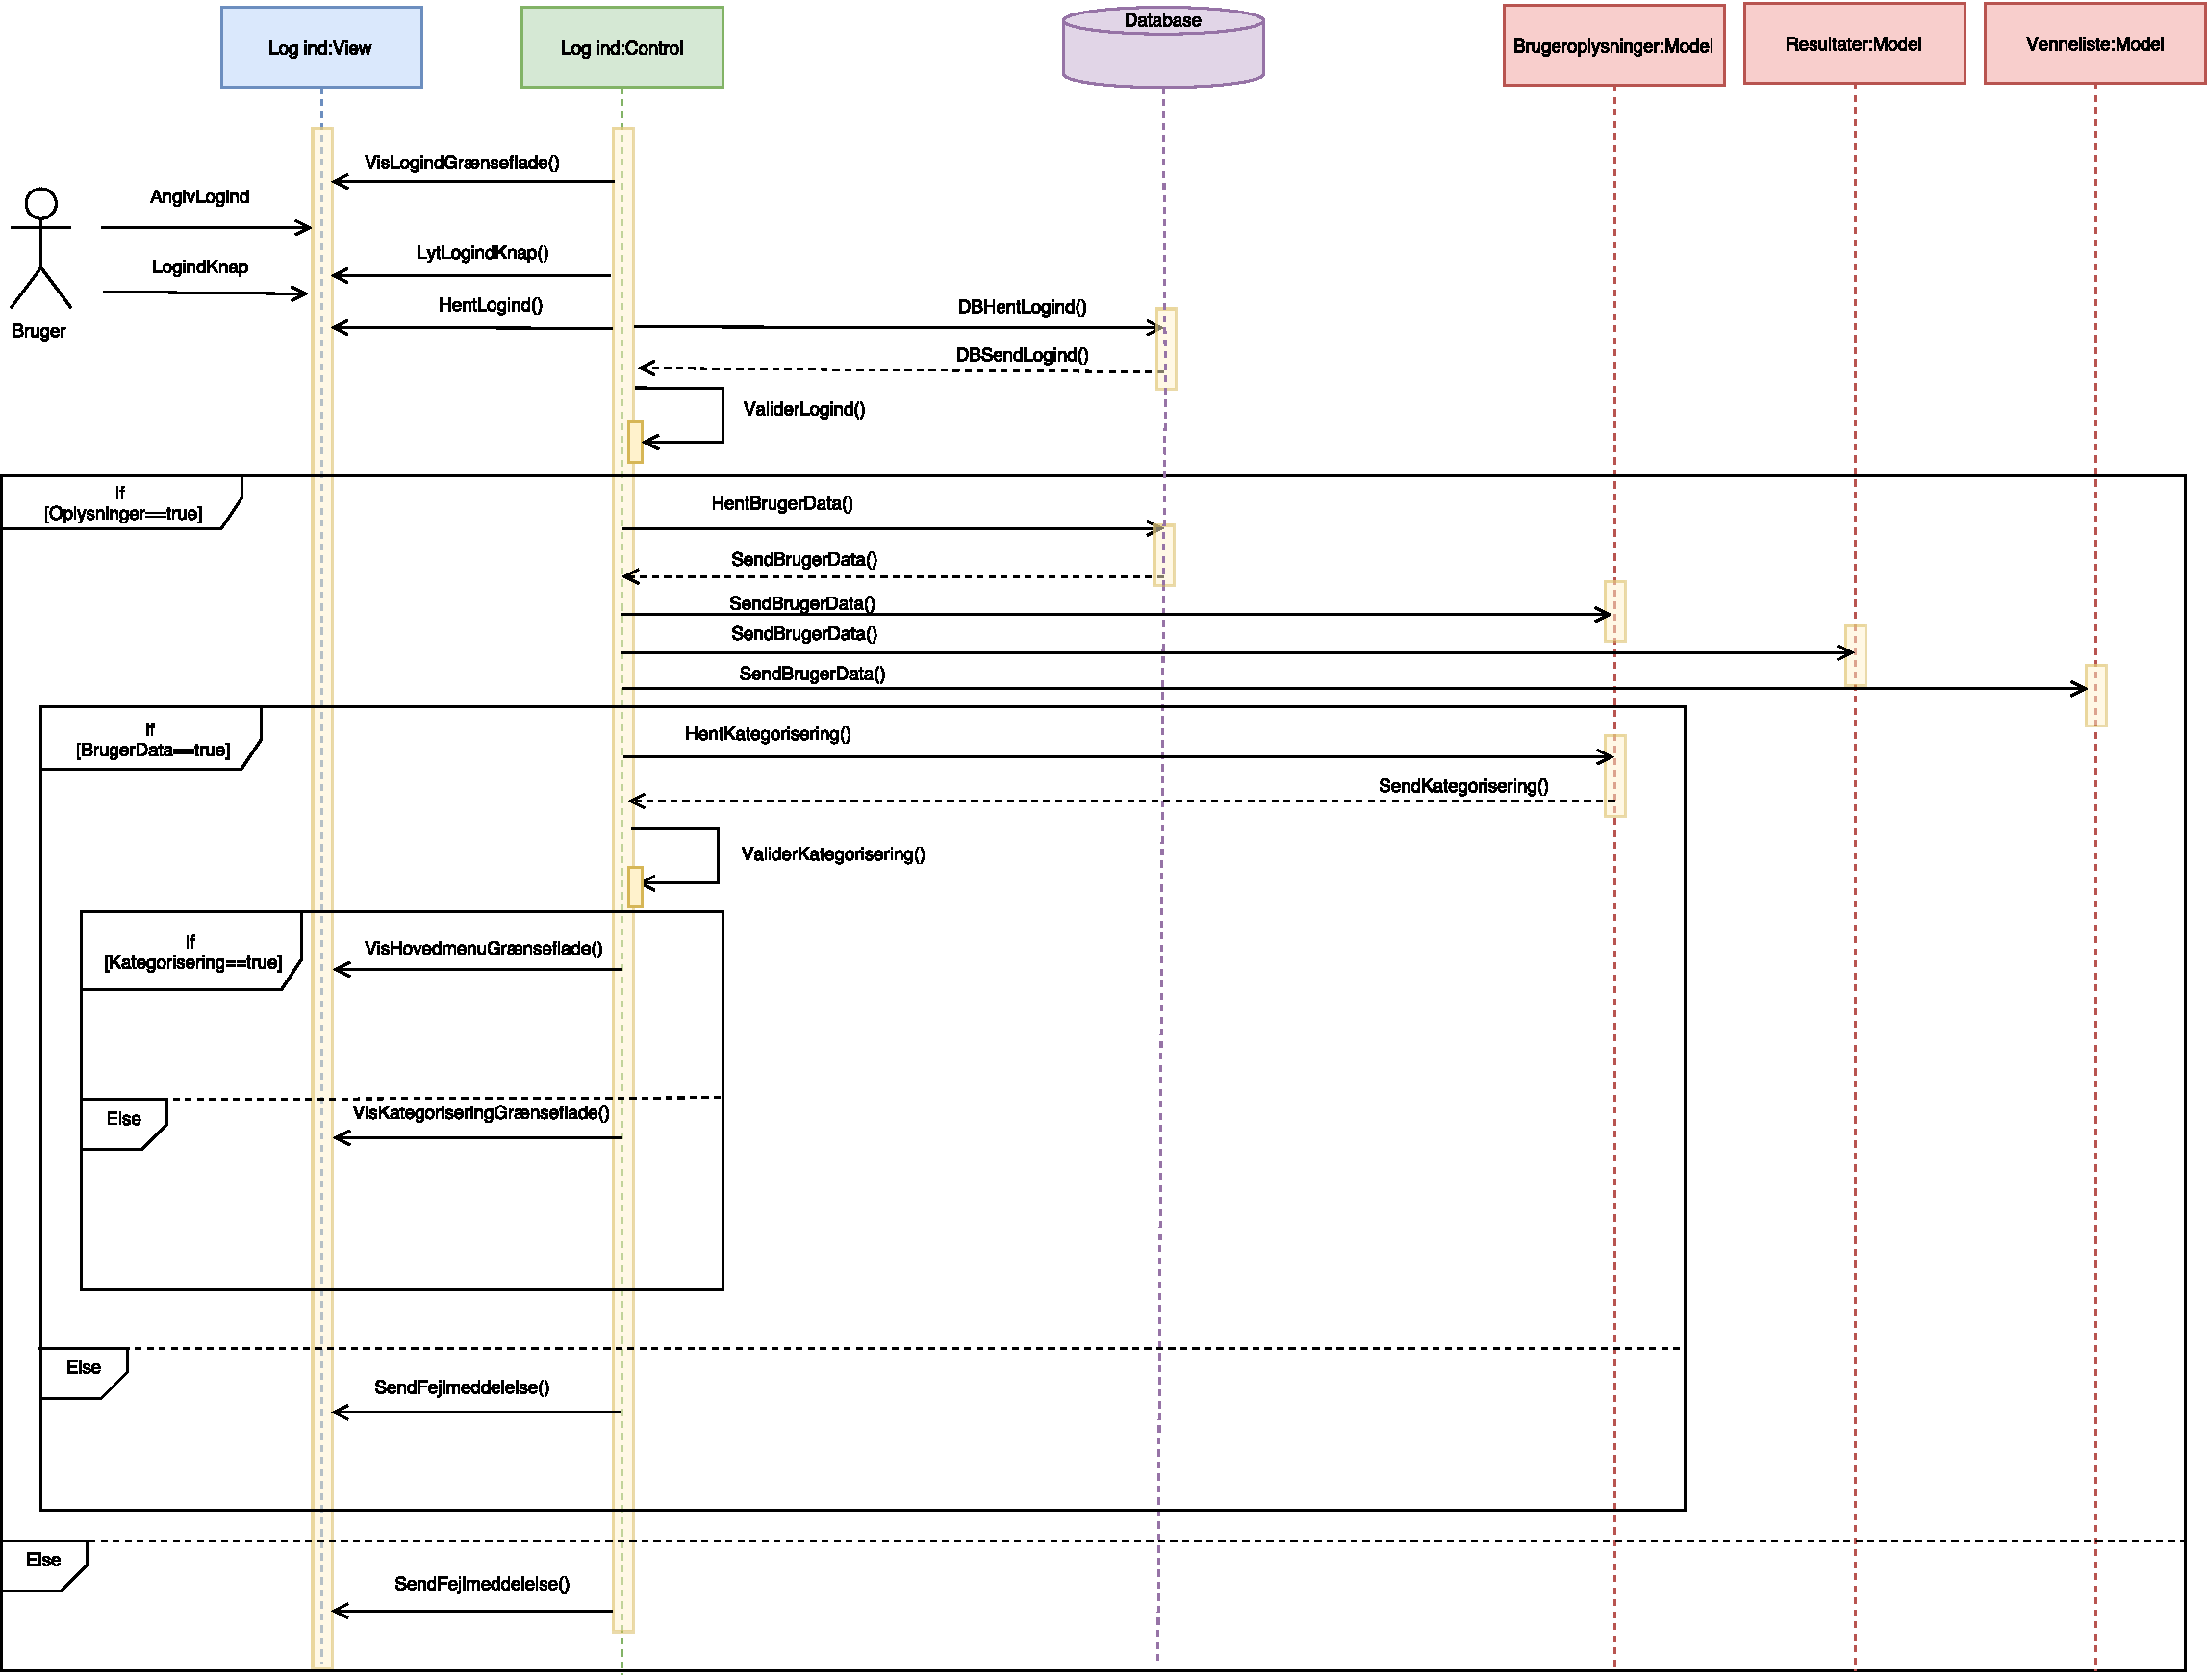
\includegraphics[width=1.55\textwidth, angle=90]{figures/Sek/SEKLogInd}
\caption{Sekvensdiagram for log ind.}
\label{fig:SEKlogind}
\end{figure}

\noindent
Det fremgår af sekvensdiagrammet, at controlleren for \textit{Log ind} starter med at vise grænsefladen for \textit{Log ind}. Dertil lytter controlleren på LogindKnap, der ved tryk henter brugerens angivne log ind-informationer. Controlleren henter ligeledes log ind-informationer passende og validerer disse i controlleren for \textit{Database}. Bekræftes log ind oprettes en entity af \textit{Brugeroplysninger}. Controlleren for \textit{Logind} henter oplysninger i databasen og sender disse til den oprettede entity. der lagrer brugeroplysninger fra databasen.Forefindes en kategorisering i de hentede brugeroplysninger startes controlleren for \textit{Hovedmenu}. Eksistere kategoriseringen ikke startes \textit{Kategorisering} controlleren. Mislykkes log ind vises en fejlmeddelelse, hvorved brugeren igen har mulighed for at indtaste log ind-oplysninger. 
